\documentclass[aspectratio=169]{beamer}

% Theme selection
\usetheme{Madrid}
\usecolortheme{whale}

% Packages
\usepackage{graphicx}
\usepackage{tikz}
\usetikzlibrary{shapes,arrows,positioning}
\usepackage{booktabs}
\usepackage{listings}
\usepackage{xcolor}
\usepackage{CJKutf8}

% Custom colors
\definecolor{codegreen}{rgb}{0,0.6,0}
\definecolor{codegray}{rgb}{0.5,0.5,0.5}
\definecolor{codepurple}{rgb}{0.58,0,0.82}
\definecolor{backcolour}{rgb}{0.95,0.95,0.92}

% Code listing style
\lstdefinestyle{mystyle}{
    backgroundcolor=\color{backcolour},   
    commentstyle=\color{codegreen},
    keywordstyle=\color{magenta},
    numberstyle=\tiny\color{codegray},
    stringstyle=\color{codepurple},
    basicstyle=\ttfamily\footnotesize,
    breakatwhitespace=false,         
    breaklines=true,                 
    captionpos=b,                    
    keepspaces=true,                 
    numbers=left,                    
    numbersep=5pt,                  
    showspaces=false,                
    showstringspaces=false,
    showtabs=false,                  
    tabsize=2
}
\lstset{style=mystyle}

\begin{document}
\begin{CJK*}{UTF8}{gbsn}

% Title Info
\title[Tarkov Weapon Optimizer]{Tarkov Weapon Mod Optimizer}
\subtitle{Automated Build Optimization using Constraint Programming}
\author{Imposs1ble嗨}
\date{\today}

\begin{frame}
    \titlepage
\end{frame}

% Section 1: Introduction
\section{Introduction}

% Slide 3: The Problem
\begin{frame}{The Problem: Complexity in Escape from Tarkov}
    \textit{Escape from Tarkov} features one of the most complex weapon modification systems in gaming.

    \vspace{0.3cm}
    \textbf{Challenges for New Players:}
    \begin{itemize}
        \item \textbf{Overwhelming scale:} 2,500+ mods, each affecting recoil, ergonomics, weight, accuracy
        \item \textbf{Nested compatibility:} Mods attach to mods (rail $\to$ mount $\to$ sight)
        \item \textbf{Combinatorial explosion:} A single AR-15 has 50+ slots, millions of valid builds
        \item \textbf{Non-obvious trade-offs:} Is a 50k grip worth it over a 5k one?
        \item \textbf{Dynamic availability:} Prices change; items locked behind trader levels, quests, and flea market access
    \end{itemize}

    \vspace{0.3cm}
    \textbf{Result:} Players spend hours theory-crafting or blindly copy ``meta builds'' without understanding trade-offs.
\end{frame}

% Slide 4: The Solution
\begin{frame}{The Solution: Automated Optimization}
    \textbf{Project Goal:}
    Create a tool that mathematically guarantees the "best" weapon build for a given set of constraints.

    \vspace{0.4cm}
    \begin{columns}
        \column{0.5\textwidth}
        \textbf{Use Cases:}
        \begin{itemize}
            \item \textit{"I have 200k roubles---what's the best M4 I can build?"}
            \item \textit{"What's the absolute lowest recoil AK, money no object?"}
            \item \textit{"I'm level 15 with LL2 traders---what can I actually buy?"}
            \item \textit{"Is spending 100k more actually worth it?"}
            \item \textit{"Show me all viable builds on a budget curve"}
        \end{itemize}

        \column{0.5\textwidth}
        \textbf{Key Capabilities:}
        \begin{itemize}
            \item \textbf{Multi-objective}: Balance recoil, ergonomics, and price
            \item \textbf{Budget-aware}: Hard limit or soft penalty on cost
            \item \textbf{Trader filtering}: Respect loyalty levels (LL1--LL4)
            \item \textbf{Flea market toggle}: Include or exclude market prices
            \item \textbf{Pareto frontier}: Visualize price vs. performance trade-offs
        \end{itemize}
    \end{columns}
\end{frame}

% Section 2: Architecture
\section{System Architecture}

% Slide: Pipeline Overview
\begin{frame}{Pipeline Overview}
    \begin{center}
    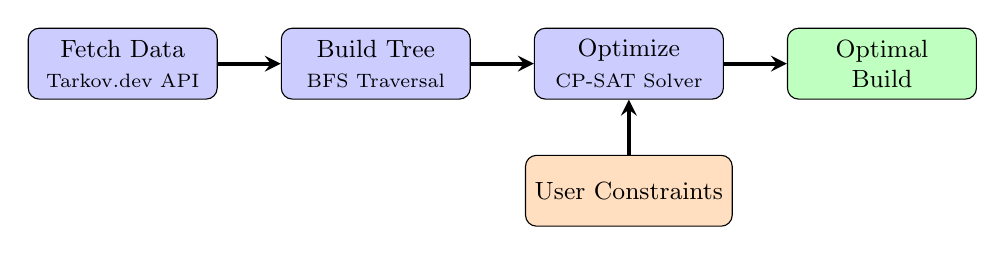
\begin{tikzpicture}[
        node distance=0.8cm,
        every node/.style={font=\small},
        box/.style={draw, rectangle, rounded corners, fill=blue!20, minimum width=2.4cm, minimum height=0.9cm, align=center},
        arrow/.style={->, thick, >=stealth, line width=1.5pt}
    ]
        % Main pipeline - horizontal
        \node[box] (fetch) {Fetch Data\\{\scriptsize Tarkov.dev API}};
        \node[box, right=of fetch] (compat) {Build Tree\\{\scriptsize BFS Traversal}};
        \node[box, right=of compat] (solve) {Optimize\\{\scriptsize CP-SAT Solver}};
        \node[box, right=of solve, fill=green!25] (result) {Optimal\\Build};

        % User input from below
        \node[box, below=0.7cm of solve, fill=orange!25] (user) {User Constraints};

        % Arrows
        \draw[arrow] (fetch) -- (compat);
        \draw[arrow] (compat) -- (solve);
        \draw[arrow] (solve) -- (result);
        \draw[arrow] (user) -- (solve);
    \end{tikzpicture}
    \end{center}
\end{frame}

% Slide 5: Fetching Data
\begin{frame}{Fetching Data}
    \begin{columns}
        \column{0.45\textwidth}
        \textbf{Tarkov.dev GraphQL API}

        \vspace{0.3cm}
        \begin{itemize}
            \item Queries all guns, mods, and compatibility rules
            \item \textbf{Up-to-date prices} from traders and flea market
            \item Trader loyalty level requirements
            \item Real-time flea market prices
            \item Local caching for speed
        \end{itemize}

        \column{0.55\textwidth}
        \begin{center}
            \includegraphics[width=\textwidth]{imgs/tarkov_dev.jpg}
        \end{center}
    \end{columns}
\end{frame}

% Slide 6a: Data Processing Pipeline
% \begin{frame}{Data Processing: From API to Item Lookup}
%     \textbf{Step 1: Raw API Data Normalization}

%     \vspace{0.2cm}
%     \begin{columns}
%         \column{0.5\textwidth}
%         \textbf{Slot Extraction Challenges:}
%         \begin{itemize}
%             \item Guns and mods have different property structures
%             \item \texttt{filters.allowedItems} can be:
%             \begin{itemize}
%                 \item List of objects: \texttt{[\{"id": "abc"\}]}
%                 \item List of strings: \texttt{["abc", "def"]}
%             \end{itemize}
%             \item Must normalize to flat list of IDs
%         \end{itemize}

%         \vspace{0.3cm}
%         \textbf{Price Validation:}
%         \begin{itemize}
%             \item Mods without valid \texttt{buyFor} offers are filtered out
%             \item Prevents selecting items that can't actually be purchased
%         \end{itemize}

%         \column{0.5\textwidth}
%         \textbf{Stat Normalization:}
%         \begin{itemize}
%             \item \textbf{Recoil modifier} formats differ:
%             \begin{itemize}
%                 \item Top-level: integer \% (e.g., \texttt{-5})
%                 \item Properties: decimal (e.g., \texttt{-0.05})
%             \end{itemize}
%             \item Normalize all to decimal format
%             \item Handle null/missing values gracefully
%         \end{itemize}

%         \vspace{0.3cm}
%         \textbf{Conflict Extraction:}
%         \begin{itemize}
%             \item \texttt{conflictingItems}: Items that can't coexist
%             \item \texttt{conflictingSlotIds}: Slots blocked by this item
%         \end{itemize}
%     \end{columns}
% \end{frame}

% Slide 6c: BFS Compatibility Tree
\begin{frame}{Building the Compatibility Tree}
    \begin{columns}
        \column{0.55\textwidth}
        \textbf{BFS Process:}
        \begin{enumerate}
            \item Start from the base weapon's slots
            \item For each slot, find all allowed items
            \item Add those items to the queue
            \item For each item, discover \textit{its} slots
            \item Repeat until no new items found
        \end{enumerate}

        \vspace{0.2cm}
        \textbf{Data Structures Built:}
        \begin{itemize}
            \item \texttt{slot\_items}: Slot $\to$ [compatible items]
            \item \texttt{slot\_owner}: Slot $\to$ parent item
            \item \texttt{item\_to\_slots}: Item $\to$ [owned slots]
        \end{itemize}

        \column{0.45\textwidth}
        \begin{center}
        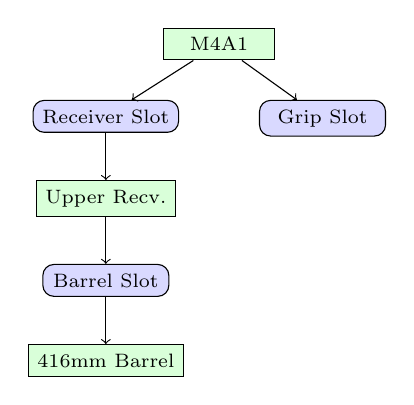
\begin{tikzpicture}[
            node distance=0.6cm,
            every node/.style={font=\scriptsize},
            slot/.style={draw, rectangle, rounded corners, fill=blue!15, minimum width=1.6cm, minimum height=0.4cm},
            item/.style={draw, rectangle, fill=green!15, minimum width=1.4cm, minimum height=0.4cm}
        ]
            \node[item] (gun) {M4A1};
            \node[slot, below left=0.5cm and -0.2cm of gun] (s1) {Receiver Slot};
            \node[slot, below right=0.5cm and -0.2cm of gun] (s2) {Grip Slot};
            \node[item, below=of s1] (upper) {Upper Recv.};
            \node[slot, below=of upper] (s3) {Barrel Slot};
            \node[item, below=of s3] (barrel) {416mm Barrel};

            \draw[->] (gun) -- (s1);
            \draw[->] (gun) -- (s2);
            \draw[->] (s1) -- (upper);
            \draw[->] (upper) -- (s3);
            \draw[->] (s3) -- (barrel);
        \end{tikzpicture}
        \end{center}
        \textit{\scriptsize Items own slots; slots contain items.}
    \end{columns}
\end{frame}

% Section 3: The Engine
\section{The Optimization Engine}

% Slide 7: What is CP-SAT?
\begin{frame}{Introduction to CP-SAT Solver}
    \textbf{CP-SAT} = \textbf{C}onstraint \textbf{P}rogramming + \textbf{SAT} (Boolean Satisfiability)

    \vspace{0.3cm}
    \begin{block}{What is it?}
        A solver from Google's OR-Tools library that finds optimal solutions to combinatorial problems by combining:
        \begin{itemize}
            \item \textbf{Constraint Programming}: Express complex rules declaratively
            \item \textbf{SAT Solving}: Efficient Boolean logic reasoning
            \item \textbf{Linear Programming}: Optimize numerical objectives
        \end{itemize}
    \end{block}

    \vspace{0.3cm}
    \textbf{Why CP-SAT for this problem?}
    \begin{itemize}
        \item Handles Boolean decisions naturally (select mod or not)
        \item Scales to thousands of variables and constraints
        \item Guarantees optimal solution (not just "good enough")
        \item Solves in milliseconds for typical weapon builds
    \end{itemize}
\end{frame}

% Slide 8: How CP-SAT Works
% \begin{frame}{How CP-SAT Works}
%     \begin{columns}
%         \column{0.5\textwidth}
%         \textbf{1. Model Definition}
%         \begin{itemize}
%             \item Create Boolean variables: $X_i \in \{0, 1\}$
%             \item Add constraints (rules)
%             \item Define objective function
%         \end{itemize}

%         \vspace{0.3cm}
%         \textbf{2. Solving Process}
%         \begin{itemize}
%             \item Propagation: Infer forced values
%             \item Search: Branch on undecided variables
%             \item Backtrack: Undo bad decisions
%             \item Prune: Skip impossible branches
%         \end{itemize}

%         \column{0.5\textwidth}
%         \textbf{3. Key Techniques}
%         \begin{itemize}
%             \item \textit{Unit Propagation}: If a constraint forces a value, apply it immediately
%             \item \textit{Conflict Learning}: Remember why branches failed to avoid repeating mistakes
%             \item \textit{Bound Tightening}: Use objective to prune suboptimal branches early
%         \end{itemize}

%         \vspace{0.3cm}
%         \textbf{Result}: Explores the search space efficiently, proving optimality.
%     \end{columns}
% \end{frame}

% Slide 9: Constraint Programming Overview
\begin{frame}{Applying CP-SAT to Weapon Builds}
    \textbf{Core Idea:} Define what a valid build looks like, let the solver find the best one.

    \vspace{0.3cm}
    \begin{block}{The Three Components}
        \begin{enumerate}
            \item \textbf{Variables}: Boolean $X_i$ for each reachable mod ($X_i = 1$ if selected)
            \item \textbf{Constraints}: Compatibility rules, budget limits, required slots
            \item \textbf{Objective}: Maximize ergonomics, minimize recoil and price
        \end{enumerate}
    \end{block}

    \vspace{0.3cm}
    The solver explores millions of mod combinations, pruning invalid builds instantly, and returns the mathematically optimal configuration.
\end{frame}

% Slide 8: Constraint 1 - Mutex
\begin{frame}{Constraint 1: Slot Mutex (One Item Per Slot)}
    \textbf{Rule:} Each slot can hold at most one item.

    \vspace{0.3cm}
    \begin{block}{Formula}
        For each slot $s$ with candidate items $\{i_1, i_2, ..., i_n\}$:
        \[
        \sum_{i \in \text{slot}_s} X_i \le 1
        \]
        where $X_i = 1$ if item $i$ is selected, $0$ otherwise.
    \end{block}

    \vspace{0.3cm}
    \textbf{Example:} A pistol grip slot can have a Zenit RK-3 \textit{or} an Ergo PSG-1, but not both simultaneously.
\end{frame}

% Slide 9: Constraint 2 - Dependency
\begin{frame}{Constraint 2: Parent Dependency}
    \textbf{Rule:} A mod can only be selected if its parent slot owner is also selected.

    \vspace{0.3cm}
    \begin{block}{Formula}
        If item $c$ (child) fits in a slot owned by item $p$ (parent):
        \[
        X_c \le X_p
        \]
        A child cannot be selected without its parent.
    \end{block}

    \vspace{0.3cm}
    \textbf{Example:} You cannot attach a foregrip to a handguard unless that handguard is installed on the weapon.

    \vspace{0.2cm}
    \begin{center}
    \textit{Gun} $\to$ \textit{Handguard} $\to$ \textit{Foregrip}
    \end{center}
\end{frame}

% Slide 10: Constraint 3 - Conflicts
\begin{frame}{Constraint 3: Conflicting Items}
    \textbf{Rule:} Some items cannot be used together (API-defined conflicts).

    \vspace{0.3cm}
    \begin{block}{Formula}
        For each conflict pair $(a, b)$ from the API:
        \[
        X_a + X_b \le 1
        \]
        At most one of the conflicting items can be selected.
    \end{block}

    \vspace{0.3cm}
    \textbf{Example:} Certain dust covers conflict with specific charging handles due to physical interference---the game prevents mounting both.
\end{frame}

% Slide 11: Constraint 4 - Required Slots
\begin{frame}{Constraint 4: Required Slots}
    \textbf{Rule:} Certain slots \textit{must} be filled for a functional weapon.

    \vspace{0.3cm}
    \begin{block}{Formula}
        For each required slot $s$:
        \[
        \sum_{i \in \text{slot}_s} X_i \ge 1
        \]
        At least one compatible item must fill the slot.
    \end{block}

    \vspace{0.3cm}
    \textbf{Vital Slots} (AR-15 platform):
    \begin{itemize}
        \item Barrel, Gas Block, Pistol Grip, Charging Handle, Receiver, Handguard
    \end{itemize}

    \vspace{0.2cm}
    Without these, the weapon cannot function in-game.
\end{frame}

% Slide 12: Budget Constraint
\begin{frame}{Constraint 5: Budget Limit}
    \textbf{Rule:} Total build cost must not exceed the player's budget.

    \vspace{0.3cm}
    \begin{block}{Formula}
        \[
        \sum_{i} \text{Price}_i \cdot X_i \le \text{Budget}
        \]
        The sum of all selected item prices must stay within budget.
    \end{block}

    \vspace{0.3cm}
    \textbf{Smart Pricing:}
    \begin{itemize}
        \item Considers trader loyalty levels (LL1--LL4)
        \item Checks flea market availability
        \item Automatically finds the cheapest source for each item
    \end{itemize}
\end{frame}

% Slide 13: Objective Function
\begin{frame}{The Objective Function}
    \textbf{Goal:} Find the build that best matches the player's priorities.

    \vspace{0.3cm}
    \begin{block}{Weighted Objective (Maximize)}
        \[
        \text{Score} = W_E \cdot \text{Ergo} - W_R \cdot \text{Recoil} - W_P \cdot \text{Price}
        \]
        \begin{itemize}
            \item $W_E$: Ergonomics weight (higher = faster ADS, less stamina drain)
            \item $W_R$: Recoil weight (lower = more controllable)
            \item $W_P$: Price weight (lower = cheaper build)
        \end{itemize}
    \end{block}

    \vspace{0.3cm}
    \textbf{Example Profiles:}
    \begin{itemize}
        \item \textit{Meta Build}: $W_R = 100, W_E = 0.5, W_P = 0$
        \item \textit{Budget Build}: $W_R = 1, W_E = 1, W_P = 0.5$
    \end{itemize}
\end{frame}

% Slide: UI - Optimizer
\begin{frame}{User Interface: Build Optimization}
    \begin{center}
        \includegraphics[width=0.9\textwidth]{imgs/page_optimize.png}
    \end{center}
\end{frame}

% Slide: Optimization Results - Recoil
\begin{frame}{Optimization Results: Min Recoil}
    \begin{center}
        \includegraphics[width=0.85\textwidth]{imgs/eg_recoil.png}
    \end{center}
\end{frame}

% Slide: Optimization Results - Ergo
\begin{frame}{Optimization Results: Max Ergo}
    \begin{center}
        \includegraphics[width=0.85\textwidth]{imgs/eg_ergo.png}
    \end{center}
\end{frame}

% Slide: Optimization Results - Balanced
\begin{frame}{Optimization Results: Balanced Build}
    \begin{center}
        \includegraphics[width=0.85\textwidth]{imgs/eg_balanced.png}
    \end{center}
\end{frame}

% Slide 14: Stat Calculations
% \begin{frame}{How Stats Are Calculated}
%     \begin{columns}
%         \column{0.5\textwidth}
%         \textbf{Ergonomics} (Additive):
%         \[
%         \text{Ergo}_{\text{final}} = \text{Ergo}_{\text{base}} + \sum_{i} \text{Ergo}_i
%         \]
%         Simply add up all mod bonuses.

%         \vspace{0.5cm}
%         \textit{Soft-capped at 100 in-game.}

%         \column{0.5\textwidth}
%         \textbf{Recoil} (Multiplicative):
%         \[
%         \text{Recoil}_{\text{final}} = \text{Recoil}_{\text{base}} \times \left(1 + \sum_{i} r_i\right)
%         \]
%         Where $r_i$ is the percentage modifier (e.g., $-0.05 = -5\%$).

%         \vspace{0.3cm}
%         \textit{Stacking suppressors gives diminishing returns.}
%     \end{columns}
% \end{frame}

% Section 4: Advanced Scalarization: Sweet Spot Mode
\section{Advanced Scalarization: Sweet Spot Mode}

% Slide: Limitation of Linear Weighted Sum
\begin{frame}{The Limitation of Linear Weighted Sum}
    \textbf{Traditional Formulation:} $\max \; W_E \cdot \text{Ergo} - W_R \cdot \text{Recoil} - W_P \cdot \text{Price}$
    
    \vspace{0.3cm}
    \begin{columns}
        \column{0.52\textwidth}
        \textbf{The Non-Convexity Problem:}
        \begin{itemize}
            \item Linear weighted sum sweeps \textbf{straight hyperplanes} across the objective space.
            \item In Tarkov, mod compatibility creates \textbf{non-convex indentations} (e.g., discrete trade-offs between heavy suppressors vs. lightweight compensators).
            \item \textbf{Mathematical Blind Spot:} Any point located inside a non-convex pocket \textbf{cannot be found by linear sums} under \textit{any} choice of weights $(W_E, W_R, W_P)$!
        \end{itemize}

        \column{0.48\textwidth}
        \begin{block}{Empirical Finding (Tarkov Datasets)}
            Across common benchmark weapons (M4A1, AK-74N, MP7A2):
            \begin{itemize}
                \item \textbf{45\%--61\%} of all Pareto-optimal builds lie in non-convex pockets!
                \item Linear weights jump directly from extreme-recoil to extreme-ergo, missing the best \textbf{"Sweet Spot"} builds.
            \end{itemize}
        \end{block}
    \end{columns}
\end{frame}

% Slide: The 3D Ideal Reference Point
\begin{frame}{The 3D Ideal Reference Point}
    \textbf{Idea:} Instead of arbitrary linear slopes, measure distance to a \textbf{Utopian Ideal Target}.
    
    \vspace{0.3cm}
    \begin{columns}
        \column{0.5\textwidth}
        \textbf{1. Utopia Ideal Point ($\mathbf{z}^*$):}
        \begin{itemize}
            \item $z^*_E = \max_{\mathbf{x}} \text{Ergo}(\mathbf{x})$ \quad (Best achievable Ergo)
            \item $z^*_R = \min_{\mathbf{x}} \text{Recoil}(\mathbf{x})$ \quad (Best achievable Recoil)
            \item $z^*_P = \min_{\mathbf{x}} \text{Price}(\mathbf{x})$ \quad (Cheapest viable build)
        \end{itemize}
        \textit{Computed instantly via 3 single-objective solves.}

        \column{0.5\textwidth}
        \textbf{2. Normalized Gap to Target ($g_i$):}
        For each objective $i \in \{E, R, P\}$:
        \[
        g_i(\mathbf{x}) = \frac{|f_i(\mathbf{x}) - z^*_i|}{\text{Range}_i} \in [0, 1]
        \]
        \begin{itemize}
            \item $g_i = 0$: Reaches the theoretical best.
            \item Dimensionless and scale-invariant across Ergo, Recoil \%, and Roubles (₽).
        \end{itemize}
    \end{columns}
\end{frame}

% Slide: Augmented Tchebycheff Formulation
\begin{frame}{Augmented Tchebycheff Scalarization}
    \textbf{Mathematical Formulation (Sweet Spot Mode):}
    \[
    \min_{\mathbf{x}, \alpha} \left( \alpha + \rho \sum_{i \in \{E, R, P\}} \lambda_i \cdot g_i(\mathbf{x}) \right)
    \]
    \[
    \text{subject to:} \quad \lambda_i \cdot g_i(\mathbf{x}) \le \alpha, \quad \forall i \in \{E, R, P\}
    \]

    \vspace{0.2cm}
    \begin{columns}
        \column{0.5\textwidth}
        \textbf{Why This Works:}
        \begin{itemize}
            \item $\alpha = \max_i (\lambda_i g_i(\mathbf{x}))$ minimizes the \textbf{worst-case deficit}.
            \item Pulls the build uniformly towards the Ideal Point from all directions.
            \item Small augmentation term $\rho \sum \lambda_i g_i$ ($\rho = 10^{-4}$) guarantees \textbf{strict Pareto optimality} (eliminates flat weak optima).
        \end{itemize}

        \column{0.5\textwidth}
        \textbf{MILP Integration Advantages:}
        \begin{itemize}
            \item Requires only \textbf{1 extra continuous variable} ($\alpha$).
            \item \textbf{Zero binary variables added} $\implies$ solve time remains $< 15\text{ms}$.
            \item Discovers non-convex sweet spots with 100\% mathematical proof of optimality.
        \end{itemize}
    \end{columns}
\end{frame}

% Slide: Geometric Intuition: Hyperplanes vs L-Contours
\begin{frame}{Geometric Intuition: Hyperplane vs. $L_\infty$ Contour}
    \begin{center}
    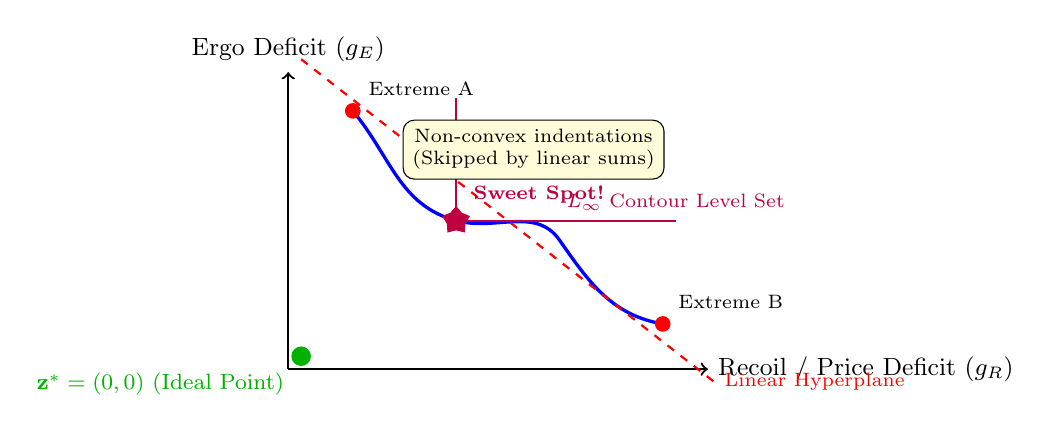
\begin{tikzpicture}[scale=0.82]
        % Axes
        \draw[->, thick] (0,0) -- (6.5,0) node[right] {\small Recoil / Price Deficit ($g_R$)};
        \draw[->, thick] (0,0) -- (0,4.6) node[above] {\small Ergo Deficit ($g_E$)};

        % Non-convex Pareto front
        \draw[very thick, blue] (1.0, 4.0) to[out=-50, in=165] (2.6, 2.3) to[out=-15, in=125] (4.2, 2.0) to[out=-55, in=170] (5.8, 0.7);

        % Ideal Point z*
        \node[fill=green!70!black, circle, inner sep=2.5pt, label={[font=\footnotesize, green!70!black]below left:$\mathbf{z}^* = (0, 0)$ (Ideal Point)}] at (0.2, 0.2) {};

        % Linear Hyperplane tangent touching extremes, missing the knee
        \draw[dashed, red, thick] (0.2, 4.8) -- (6.6, -0.2) node[right, font=\scriptsize, red] {Linear Hyperplane};
        \node[fill=red, circle, inner sep=2pt, label={[font=\scriptsize]above right:Extreme A}] at (1.0, 4.0) {};
        \node[fill=red, circle, inner sep=2pt, label={[font=\scriptsize]above right:Extreme B}] at (5.8, 0.7) {};

        % Tchebycheff L-contour
        \draw[thick, purple] (2.6, 4.2) -- (2.6, 2.3) -- (6.0, 2.3) node[above, font=\scriptsize, purple] {$L_\infty$ Contour Level Set};
        \node[fill=purple, star, star points=5, inner sep=2.5pt, label={[font=\scriptsize, purple]above right:\textbf{Sweet Spot!}}] at (2.6, 2.3) {};

        \node[draw, rounded corners, fill=yellow!15, font=\scriptsize, align=center] at (3.8, 3.4) {Non-convex indentations\\(Skipped by linear sums)};
    \end{tikzpicture}
    \end{center}
    \textbf{Key Takeaway:} Straight lines bridge across concave regions, while L-shaped Chebyshev contours penetrate deep into the "knee" to find balanced builds.
\end{frame}

% Section 5: Aiming Physics & EvoErgo Optimization
\section{Aiming Physics \& EvoErgo Optimization}

% Slide: In-Game ADS Physics Problem
\begin{frame}{In-Game ADS Physics \& The Overswing Problem}
    \textbf{The Real-World Tarkov Combat Dilemma:}
    \begin{itemize}
        \item High Ergonomics speeds up Aim-Down-Sights (ADS) transition and reduces arm stamina drain.
        \item However, heavy weapon weight introduces \textbf{rotational momentum and inertia}.
    \end{itemize}

    \vspace{0.3cm}
    \begin{columns}
        \column{0.5\textwidth}
        \begin{block}{What is Sight Overswing?}
            When quickly snapping to aim, a weapon whose weight exceeds its ergonomic handling limit will \textbf{sway past the target reticle} before settling.
            \begin{itemize}
                \item Causes missed first shots in high-tempo CQB.
                \item A 100-ergo, 7.5\,kg build overswings violently.
                \item A 65-ergo, 3.2\,kg build snaps instantly and stably.
            \end{itemize}
        \end{block}

        \column{0.5\textwidth}
        \begin{center}
        \textit{"Raw Ergonomics is misleading without accounting for weapon weight."}
        
        \vspace{0.3cm}
        \textbf{Community Research:}\\
        SpaceMonkey37 \& EFTForge established the empirical relationship between Ergonomics, Weight, and Overswing.
        \end{center}
    \end{columns}
\end{frame}

% Slide: Quadratic EvoErgoDelta (EED)
\begin{frame}{The Quadratic EvoErgoDelta ($\text{EED}$) Metric}
    \textbf{Community Formulation (SpaceMonkey37 / EFTForge):}
    \[
    \text{EED} = \left[ 100 - 0.015 \cdot (100 - \text{Ergo})^2 \right] - 15 \cdot \text{Weight}_{\text{kg}}
    \]

    \vspace{0.2cm}
    \begin{columns}
        \column{0.5\textwidth}
        \textbf{The Physical Meaning of $\text{EED}$:}
        \begin{itemize}
            \item \textcolor{green!60!black}{\textbf{$\text{EED} \ge 0$ (Zero Overswing)}}: Weight is within the ergonomic threshold; sights snap cleanly on target.
            \item \textcolor{red!80!black}{\textbf{$\text{EED} < 0$ (Overswing Detected)}}: Weapon inertia causes crosshair sway upon entering ADS.
        \end{itemize}

        \column{0.5\textwidth}
        \textbf{Linearized Approximation (EvoErgo):}
        \[
        \text{EvoErgo} = \min(100, \text{Ergo}) - 15 \cdot \text{Weight}_{\text{kg}}
        \]
        \begin{itemize}
            \item Standard community linear score displayed in results overview cards.
            \item Balances ergonomics and weight directly at a 1:15 kg exchange rate.
        \end{itemize}
    \end{columns}
\end{frame}

% Slide: Linearizing Quadratic EED via Tangent k-Sweep
\begin{frame}{Solving Non-Linear EED: The Tangent $k$-Sweep Solver}
    \textbf{Optimization Challenge:} $\text{EED}$ is quadratic and non-linear, but LP/MIP solvers require linear objectives for sub-millisecond execution.

    \vspace{0.3cm}
    \textbf{Tangent Exchange Rate:} The marginal value of ergonomics varies with current ergo $E$:
    \[
    k(E) = \frac{\partial \text{EED}}{\partial E} = 0.03 \cdot (100 - E) + 15 \quad (\text{Exchange slope } \Delta W / \Delta E)
    \]

    \vspace{0.2cm}
    \begin{block}{The Tangent $k$-Sweep Algorithm (\texttt{solveEvoErgo})}
        \begin{enumerate}
            \item Run candidate linear solves across benchmark exchange rates $k \in \{15.0, 10.0, 7.5, 5.6\}$ and $k(E_0)$.
            \item Obtain integer-feasible candidate loadouts $\mathbf{x}^{(1)}, \mathbf{x}^{(2)}, \dots, \mathbf{x}^{(m)}$.
            \item Evaluate exact quadratic $\text{EED}(\mathbf{x}^{(j)})$ on each candidate.
            \item Return the global maximum $\mathbf{x}^* = \arg\max \text{EED}(\mathbf{x}^{(j)})$ in $< 10\text{ms}$.
        \end{enumerate}
    \end{block}
\end{frame}

% Slide: Prevent Overswing Hard Constraint
\begin{frame}{Hard Constraint: Prevent Sight Overswing}
    \textbf{Requirement:} Ensure the optimized weapon guarantees \textbf{Zero Overswing} ($\text{EED} \ge 0$).
    \[
    \text{Weight}_{\text{kg}} \le \text{Threshold}(E_{\text{eff}}) = \frac{100 - 0.015 \cdot (100 - E_{\text{eff}})^2}{15}
    \]

    \vspace{-0.1cm}
    \begin{columns}
        \column{0.55\textwidth}
        \begin{center}
        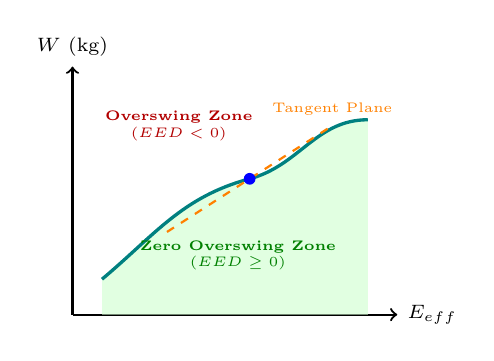
\begin{tikzpicture}[scale=0.75]
            \draw[->, thick] (0,0) -- (5.5,0) node[right] {\scriptsize $E_{\text{eff}}$};
            \draw[->, thick] (0,0) -- (0,4.2) node[above] {\scriptsize $W$ (kg)};

            \fill[green!15, opacity=0.8] (0.5, 0) -- (0.5, 0.6) to[out=40, in=195] (3.0, 2.3) to[out=15, in=180] (5.0, 3.3) -- (5.0, 0) -- cycle;
            \draw[very thick, teal] (0.5, 0.6) to[out=40, in=195] (3.0, 2.3) to[out=15, in=180] (5.0, 3.3);

            \node[font=\tiny, green!50!black, align=center] at (2.8, 1.0) {\textbf{Zero Overswing Zone}\\($\text{EED} \ge 0$)};
            \node[font=\tiny, red!70!black, align=center] at (1.8, 3.2) {\textbf{Overswing Zone}\\($\text{EED} < 0$)};

            \draw[dashed, thick, orange] (1.6, 1.4) -- (4.4, 3.2) node[above, font=\tiny, orange] {Tangent Plane};
            \node[fill=blue, circle, inner sep=1.5pt] at (3.0, 2.3) {};
        \end{tikzpicture}
        \end{center}

        \column{0.45\textwidth}
        \textbf{Tangent Cutting Planes:}
        \begin{itemize}
            \item Replaces the quadratic curve with first-order tangent cuts:
            \[
            W \le T(E_0) + T'(E_0)(E - E_0)
            \]
            \item Convex upper bound: zero binary variables needed, solving in $< 15\text{ms}$.
        \end{itemize}
    \end{columns}
\end{frame}

% Slide: Equipment Ergonomics Modifier (b)
\begin{frame}{Equipment Ergonomics Modifier ($b$)}
    \textbf{Real Combat Scenario:} Body armor, armored rigs, helmets, and backpacks reduce your effective ergonomics.

    \vspace{0.3cm}
    \begin{block}{Effective Ergonomics Loadout Formula}
        \[
        E_{\text{eff}} = E_{\text{weapon}} \cdot (1 + b), \quad b \in [-0.40, \; 0.00]
        \]
        \begin{itemize}
            \item $b$: Total equipment ergo penalty percentage from player loadout.
            \item Example: A heavy Tier-6 Zabralo armor ($b = -28\%$) + Altyn helmet ($b = -7\%$) $\implies b = -35\%$.
        \end{itemize}
    \end{block}

    \vspace{0.3cm}
    \textbf{Player Benefit:} The optimizer automatically adjusts the overswing threshold to account for your armor, guaranteeing that the build snaps with zero sway in full raid gear.
\end{frame}

% Section 6: Key Features
\section{Key Features}
% Slide: Gunsmith Task Solver
\begin{frame}{Gunsmith Task Solver}
    \textbf{Problem:} Gunsmith quests require building weapons to exact specifications.

    \vspace{0.2cm}
    \begin{columns}
        \column{0.5\textwidth}
        \textbf{Task Definition (JSON):}
        \begin{itemize}
            \item Target weapon name
            \item Stat constraints:
            \begin{itemize}
                \item Min ergonomics, max recoil
                \item Min magazine capacity
                \item Max weight, min sighting range
            \end{itemize}
            \item Required specific items
            \item Required categories (e.g., ``Silencer'')
        \end{itemize}

        \column{0.5\textwidth}
        \textbf{How It Works:}
        \begin{enumerate}
            \item Load task from \texttt{tasks.json}
            \item Convert requirements to constraints:
            \begin{itemize}
                \item Required items $\to$ $X_i = 1$
                \item Categories $\to$ $\sum_{i \in \text{cat}} X_i \ge 1$
                \item Stats $\to$ hard bounds
            \end{itemize}
            \item Objective: minimize price
            \item Solver finds cheapest valid build
        \end{enumerate}
    \end{columns}

    \vspace{0.2cm}
    \textbf{Result:} Automatically solves all 25 Gunsmith quests with optimal (cheapest) builds.
\end{frame}

% Slide: Gunsmith List
\begin{frame}{Gunsmith Task List}
    \begin{center}
        \includegraphics[width=0.9\textwidth,height=0.75\textheight,keepaspectratio]{imgs/eg_gunsmith.png}
    \end{center}
\end{frame}

% Slide: Gunsmith Details
\begin{frame}{Gunsmith Solution Details}
    \begin{center}
        \includegraphics[width=0.9\textwidth,height=0.75\textheight,keepaspectratio]{imgs/eg_gunsmith_2.png}
    \end{center}
\end{frame}

% Slide 9: Pareto Frontier
\begin{frame}{Pareto Frontier Analysis}
    \textbf{What is it?}
    \begin{itemize}
        \item A curve showing the trade-off between two conflicting goals (e.g., Price vs. Recoil).
    \end{itemize}

    \begin{center}
    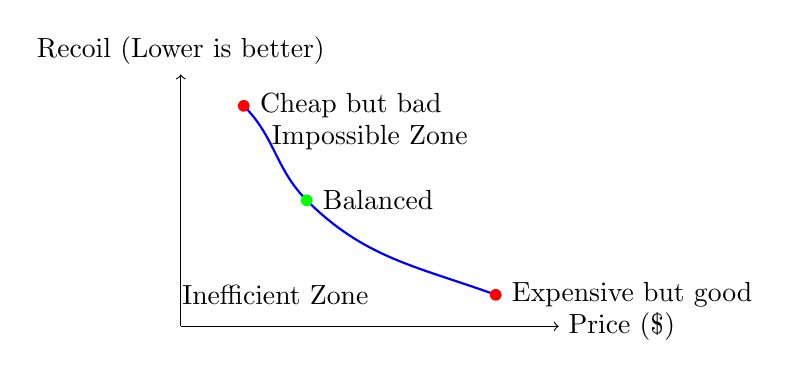
\begin{tikzpicture}[scale=0.8]
        \draw[->] (0,0) -- (6,0) node[right] {Price (\$)};
        \draw[->] (0,0) -- (0,4) node[above] {Recoil (Lower is better)};
        
        \draw[thick, blue] (1, 3.5) to[out=-45, in=135] (2, 2) to[out=-45, in=160] (5, 0.5);
        
        \node[fill=red, circle, inner sep=1.5pt, label=right:Cheap but bad] at (1, 3.5) {};
        \node[fill=green, circle, inner sep=1.5pt, label=right:Balanced] at (2, 2) {};
        \node[fill=red, circle, inner sep=1.5pt, label=right:Expensive but good] at (5, 0.5) {};
        
        \node at (3, 3) {Impossible Zone};
        \node at (1.5, 0.5) {Inefficient Zone};
    \end{tikzpicture}
    \end{center}
    
    \textbf{Why use it?} Allows users to see if spending an extra 50k Roubles actually gives a significant benefit.
\end{frame}

% Slide: Pareto Visualization
\begin{frame}{Pareto Frontier Visualization}
    \begin{center}
        \includegraphics[width=0.9\textwidth,height=0.75\textheight,keepaspectratio]{imgs/page_pareto.png}
    \end{center}
\end{frame}

% Slide: Future Work
\begin{frame}{Future Work \& Unimplemented Features}
    \begin{itemize}
        \item \textbf{Hidden Weapon Stats}: Currently unable to retrieve hidden weapon stats, such as recoil angle.
        \item \textbf{Trader Barters}: Currently unable to retrieve trader barter items and their calculated prices.
    \end{itemize}
\end{frame}

% Section 7: Conclusion
\section{Conclusion}

% Acknowledgements
\begin{frame}{Acknowledgements}
    \begin{center}
        \textbf{\Large Data Source}

        \vspace{0.2cm}
        \includegraphics[height=0.9cm]{logos/tarkov-dev-logo.png}

        \vspace{0.1cm}
        Open-source GraphQL API for Escape from Tarkov

        \vspace{0.4cm}
        \textbf{\Large AI Coding Assistants}

        \vspace{0.3cm}
        \begin{tabular}{c @{\hspace{1cm}} c @{\hspace{1cm}} c}
            \includegraphics[height=1.1cm]{logos/claude-color.png} &
            \includegraphics[height=1.1cm]{logos/gemini-color.png} &
            \includegraphics[height=1.1cm]{logos/minimax-color.png} \\[0.2cm]
            \textbf{Claude Code} & \textbf{Gemini CLI} & \textbf{MiniMax} \\[0.1cm]
            Anthropic & Google & MiniMax \\
        \end{tabular}

        \vspace{0.3cm}
        \textit{All the AI assistants helped me with code generation, debugging, and documentation}
    \end{center}
\end{frame}

\end{CJK*}
\end{document}
